\documentclass[aspectratio=169]{beamer}
% \usepackage{pgfpages}
% \pgfpagesuselayout{4 on 1}[a4paper,landscape,border shrink=5mm]
\usepackage{tikz}
\usetikzlibrary{shapes, backgrounds, arrows, positioning}
\usepackage{pgfplots}
\usepackage{listings}
\usepackage[utf8,latin1]{inputenc}
\usepackage[style = apa, backend = biber, natbib = true]{biblatex}
\addbibresource{../../literature/lit.bib}

\makeatletter \def\newblock{\beamer@newblock} \makeatother

\beamertemplatenavigationsymbolsempty
\setbeamertemplate{itemize items}[circle]
\setbeamertemplate{section in toc}[circle]
\mode<beamer>{\setbeamercolor{math text displayed}{fg=iwmgray}}
\setbeamercolor{block body}{bg=iwmorange!50!white}
\setbeamercolor{block title}{fg=white, bg=iwmorange}

% Definitions for biblatex
\setbeamercolor{bibliography entry note}{fg=iwmgray}
\setbeamercolor{bibliography entry author}{fg=iwmgray}
\setbeamertemplate{bibliography item}{}

\definecolor{iwmorange}{RGB}{255,105,0}
\definecolor{iwmgray}{RGB}{67,79,79}
\definecolor{iwmblue}{RGB}{60,180,220}
\definecolor{iwmgreen}{RGB}{145,200,110}
\definecolor{iwmpurple}{RGB}{120,0,75}

\setbeamercolor{title}{fg=iwmorange}
\setbeamercolor{frametitle}{fg=iwmorange}
\setbeamercolor{structure}{fg=iwmorange}
\setbeamercolor{normal text}{fg=iwmgray}
\setbeamercolor{author}{fg=iwmgray}
\setbeamercolor{date}{fg=iwmgray}
\color{white}

\title{Generalized linear models (GLM)}
\author{Nora Wickelmaier}
\date{Last modified: \today}

\newcommand{\vect}[1]{\mathbf{#1}}
\newcommand{\mat}[1]{\mathbf{#1}}
\newcommand{\gvect}[1]{\boldsymbol{#1}}
\newcommand{\gmat}[1]{\boldsymbol{#1}}

\lstset{language = R,%
  basicstyle = \ttfamily\color{iwmgray},
  frame = single,
  rulecolor = \color{iwmgray},
  commentstyle = \slshape\color{iwmgreen},
  keywordstyle = \bfseries\color{iwmgray},
  identifierstyle = \color{iwmpurple},
  stringstyle = \color{iwmblue},
  numbers = none,%left,numberstyle = \tiny,
  basewidth = {.5em, .4em},
  showstringspaces = false,
  emphstyle = \color{red!50!white}}

\pgfmathdeclarefunction{gauss}{2}{%
  \pgfmathparse{1/(#2*sqrt(2*pi))*exp(-((x-#1)^2)/(2*#2^2))}%
}

\AtBeginSection[]{
  \frame{
    \tableofcontents[sectionstyle=show/hide, subsectionstyle=show/show/hide]}}

\setbeamertemplate{headline}{
 \begin{beamercolorbox}{section in head}
   \vskip5pt\insertsectionnavigationhorizontal{\paperwidth}{}{}\vskip2pt
 \end{beamercolorbox}
}

\setbeamertemplate{footline}{\vskip-2pt\hfill\insertframenumber$\;$\vskip2pt}

\begin{document}

\begin{frame}{}
\thispagestyle{empty}
\titlepage
\end{frame}

\begin{frame}{Outline}
\tableofcontents
\end{frame}

\begin{frame}{Linear regression}
  \begin{columns}
    \begin{column}{.5\textwidth}
      \begin{itemize}
        \item Constant change in predictor leads to constant change in response
          variable\\[2ex]
        \item[$\to$] Implies that response variable can vary indefinitely in both
              directions (or only varies by a relative small amount)
      \end{itemize}
    \end{column}
    \begin{column}{.6\textwidth}
        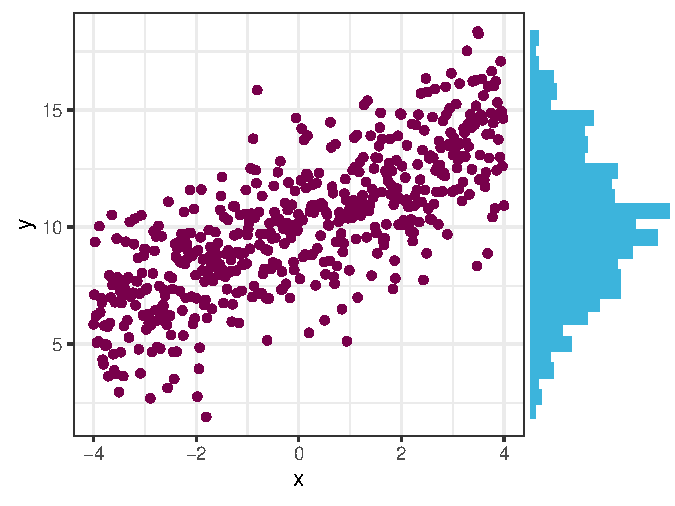
\includegraphics[scale=.7]{../figures/glm_lin}
    \end{column}
  \end{columns}
\end{frame}

\begin{frame}{Extending linear regression for arbitrary distributions}
  \begin{columns}
    \begin{column}{.5\textwidth}
      \begin{itemize}
    \item Generalized linear models allow for response variables that have
      \textbf{arbitrary distributions}
    \item[$\to$] An arbitrary function of the response variable (the link function)
      varies linearly with the predictors (rather than assuming that the
          response itself must vary linearly)
      \end{itemize}
    \end{column}
    \begin{column}{.6\textwidth}
        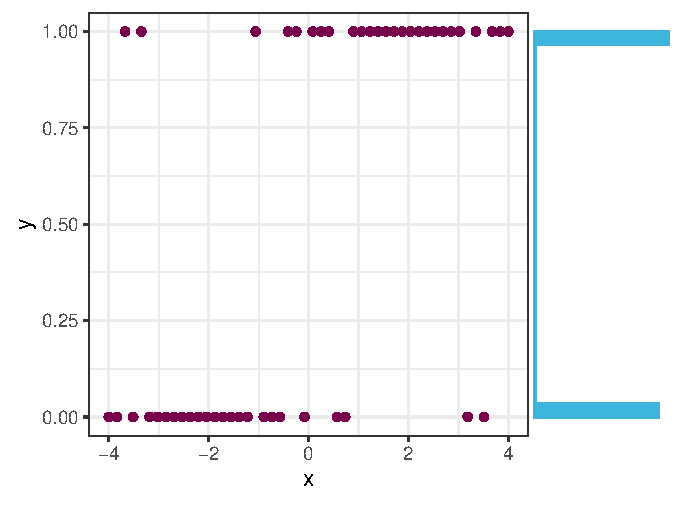
\includegraphics[scale=.7]{../figures/glm_bin}
    \end{column}
  \end{columns}
\end{frame}


\begin{frame}[allowframebreaks]{Intuition}
  \vspace{.7cm}
  \begin{itemize}
    \item Example 1: Model that predicts probability of making yes/no
      choice
      \begin{itemize}
        \item How likely is it for a given person to go to the beach as a
          function of temperature?
        \item A model might predict, for example, that a change in 10 degrees
          makes a person two times more or less likely to go to the beach
        \item That means the odds are doubling: from 2:1 odds to 4:1 odds
          and so on
      \end{itemize}
  \end{itemize}
  \vspace{.5cm}

  \begin{tabular}{|l|c|c|c|}
    \hline
    Temperature &  $10^{\circ} C$  &  $20^{\circ} C$ & $30^{\circ} C$  \\
    \hline
    &
    
\includegraphics[width = 1cm]{../figures/tanning}
    
\includegraphics[width = 1cm]{../figures/relax} &
    
\includegraphics[width = 1cm]{../figures/tanning}
    
\includegraphics[width = 1cm]{../figures/tanning}
    
\includegraphics[width = 1cm]{../figures/relax} &
    
\includegraphics[width = 1cm]{../figures/tanning}
    
\includegraphics[width = 1cm]{../figures/tanning}
    
\includegraphics[width = 1cm]{../figures/tanning}
    
\includegraphics[width = 1cm]{../figures/tanning}
    
\includegraphics[width = 1cm]{../figures/relax} \\
    Odds & $1:1$  & $2:1$ & $4:1$ \\
    \hline
  \end{tabular}

  \vfill
{\scriptsize
  \url{https://www.flaticon.com/free-icons/tanning},
  \url{https://www.flaticon.com/free-icons/work}
  }
  \framebreak
  
  \begin{itemize}
      \item Example 2: Model that predicts a certain count
      \begin{itemize}
        \item A model might predict a constant rate of increased beach
          attendance (e.g., an increase of 10 degrees leads to a doubling in
          beach attendance, and a drop of 10 degrees leads to a halving in
          attendance)
        \item This prediction would be independent of the size of the beach
      \end{itemize}
  \end{itemize}
  \vspace{.5cm}

  \begin{tabular}{|l|c|c|}
    \hline
    Temperature &  $20^{\circ} C$ & $30^{\circ} C$  \\
    \hline
    &
    
\includegraphics[width = 1cm]{../figures/tanning}
    
\includegraphics[width = 1cm]{../figures/tanning}
    
\includegraphics[width = 1cm]{../figures/tanning}
    
\includegraphics[width = 1cm]{../figures/tanning}
    
\includegraphics[width = 1cm]{../figures/tanning}
    &
    
\includegraphics[width = 1cm]{../figures/tanning}
    
\includegraphics[width = 1cm]{../figures/tanning}
    
\includegraphics[width = 1cm]{../figures/tanning}
    
\includegraphics[width = 1cm]{../figures/tanning}
    
\includegraphics[width = 1cm]{../figures/tanning} \\
    & &
    
\includegraphics[width = 1cm]{../figures/tanning}
    
\includegraphics[width = 1cm]{../figures/tanning}
    
\includegraphics[width = 1cm]{../figures/tanning}
    
\includegraphics[width = 1cm]{../figures/tanning}
    
\includegraphics[width = 1cm]{../figures/tanning} \\
    Number & 5  & 10 \\
    \hline
  \end{tabular}

  \vspace{.5cm}
{\scriptsize \url{https://en.wikipedia.org/wiki/Generalized_linear_model}}

\end{frame}

\begin{frame}[fragile]{Generalized linear models}
  \begin{itemize}
    \item A generalized linear model is defined by
\[
  g(E(y)) = \beta_0 + \beta_1 x_1 + \beta_2 x_2 + \cdots + \beta_k x_k,
\]
where $g()$ is the link function that links the mean to the linear predictor
\item The response $y$ is assumed to be independent and to follow a distribution
  from the exponential family

\item In R, a GLM is fitted by

  \begin{lstlisting}
  glm(y ~ x1 + x2 + ... + xk, family(link), data)
\end{lstlisting}
  \end{itemize}
\end{frame}

\begin{frame}[fragile]{Families}
  \begin{itemize}
    \item Each response distribution admits a variety of link functions to
      connect the mean with the linear predictor:

  \begin{lstlisting}
## Family name       Link functions
   binomial          logit, probit, log, cloglog
   gaussian          identity, log, inverse
   Gamma             identity, inverse, log
   inverse.gaussian  1/mu^2, identity, inverse, log
   poisson           log, identity, sqrt

   quasi             logit, probit, cloglog, identity,
                     inverse, log, 1/mu^2, sqrt
\end{lstlisting}
\item A GLM is a specific combination of a response distribution, a link
  function, and a linear predictor
  \end{itemize}
\end{frame}

\section{Logistic regression}

\begin{frame}{Binomial regression}
  \begin{itemize}
    \item Logit or probit models are special cases of GLMs for binomial
      response variables
    \item Artificial example: congenital eye disease
  \end{itemize}
\begin{columns}[c]
\begin{column}{6cm}
  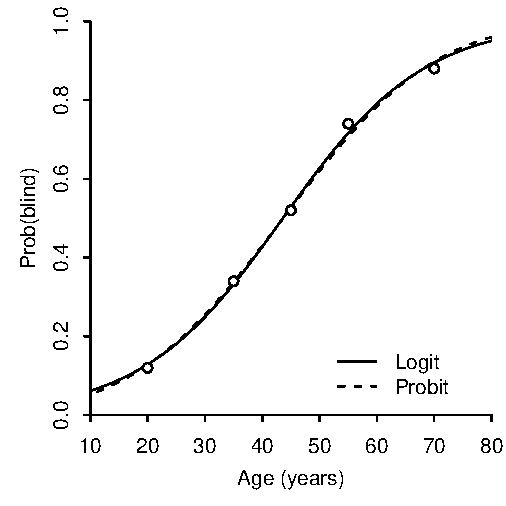
\includegraphics[scale=.7]{../figures/glm}
\end{column}
\begin{column}{5cm}
Logit model
\[
  \log\frac{p}{1 - p} = \beta_0 + \beta_1 AGE
\]
Probit model
\[
  \Phi^{-1}(p) = \beta_0 + \beta_1 AGE
\]
\end{column}
\end{columns}
\end{frame}


\begin{frame}{Probabilities, Odds, Logit}
  \begin{columns}
    \begin{column}{.35\textwidth}
\small
  Probabilities, Odds and Logits are measures for the tendency that an event
  occurs
  \begin{itemize}
    \item $Odds = \dfrac{p}{1 - p}$\\
      number of expected events per complementary event
    \item $logit = \log(Odds)$\\
      natural logarithm of odds
  \end{itemize} 
    \end{column}
    \begin{column}{.65\textwidth}
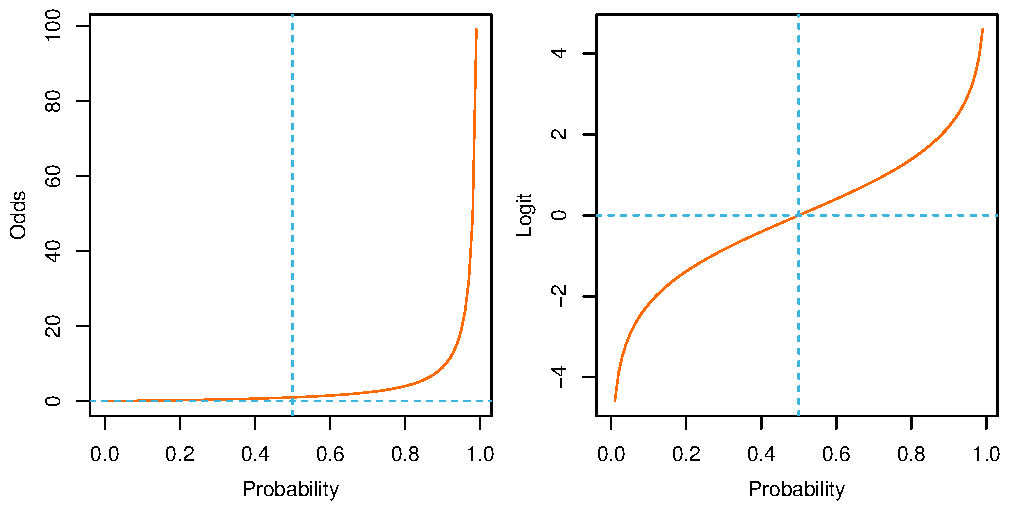
\includegraphics[scale=.55]{../figures/oddslogit}
    \end{column}
  \end{columns}
  \begin{center}
\begin{tabular}{|cccccccc|}
\hline
$p$       & 0.01    & 0.05 & 0.33 & 0.50 & 0.66 & 0.95 & 0.99 \\
Odds        & 1/99    & 1/19 & 0.49 & 1 & 1.94 & 19 & 99 \\
logit $p$ & $-$4.60 & $-$2.94 & $-$0.71 & 0 & 0.66 & 2.94 & 4.60 \\
\hline
\end{tabular}
  \end{center}
\end{frame}


\begin{frame}{Logit model / logistic regression}
  \begin{itemize}
    \item We want to model the probability of $y$ with the logistic
      function
  \begin{equation*}
    p(y) = \frac{1}{1 + e^{-z}}~~\text{  with } y \sim Binom(n, p)
  \end{equation*}
    \item How do we get the logit model $\log\frac{p}{1 - p} =
      \beta_0 + \beta_1 x$ from that?
  \end{itemize}\pause
      \begin{align*}
        \log\left(\frac{p}{1 - p}\right) = \log(p) - \log(1-p) 
        & = \log\left(\frac{1}{1 + e^{-z}}\right) - \log\left(1 - \frac{1}{1 + e^{-z}}\right) \\
        & = \log(1) - \log(1 + e^{-z}) - \log(e^{-z}) + \log(1 + e^{-z}) \\
        & = -\log(e^{-z})\\
        & = z := \beta_0 + \beta_1 x
      \end{align*}
     with \color{iwmorange}{$1 - \frac{1}{1 + e^{-z}} = \frac{e^{-z}}{1 + e^{-z}}$}
\end{frame}

\begin{frame}{Refresher: Logarithm rules}

\begin{tabular}{p{2cm}l}
  Product:  & $\log(xy)=\log x+\log y$ \\
  &\\
  Quotient: & $\log\!{\frac {x}{y}}=\log x-\log y$ \\
  &\\
  Power:    & $\log\left(x^{p}\right)=p\log x$ \\
  &\\
  Root:     & $\log{\sqrt[{p}]{x}}={\frac {\log x}{p}}$ \\
\end{tabular}

\end{frame}

\begin{frame}[fragile]{Fitting binomial regression models}
\begin{lstlisting}
dat <- data.frame(x = c(20, 35, 45, 55, 70),
                  n = rep(50, 5),
                  y = c(6, 17, 26, 37, 44))

glml <- glm(cbind(y, n - y) ~ x, family = binomial, data = dat)
glmp <- glm(cbind(y, n - y) ~ x, family = binomial(probit), data = dat)

# Parameter estimates
summary(glml)

# Interpretation as odds ratio
exp(coef(glml))
# --> Odds of going blind are increased by a factor
# of 1.08 when age increases by one year
\end{lstlisting}
\end{frame}

\begin{frame}[fragile]{Goodness of fit and predictions}
\begin{lstlisting}
# Compare to saturated model
glms <- glm(cbind(y, n - y) ~ factor(x), family = binomial, data = dat)

# Likelihood ratio test
anova(glml, glms, test = "Chisq")

# Predictions based on new observations (see ?predict.glm)
newx <- 0:100
predict(glml, newdata = data.frame(x = newx), type = "response")
\end{lstlisting}
\end{frame}

\begin{frame}[fragile]{}
  \begin{block}{Exercise}
    \begin{itemize}
\item In a psychophysical experiment two LEDs are presented to a
  subject: a standard with 40\,cd/m$^2$ and a comparison with varying
        intensities
    \item The subject is supposed to say which stimulus is
      brighter; each comparison is presented 40 times
        \vspace{.2cm}
\begin{center}
\begin{tabular}{l|rrrrrrr}
x (cd/m$^2$)  & 37 & 38 & 39 & 40 & 41 & 42 & 43 \\ \hline
y (positiv)   &  2 &  3 & 10 & 25 & 34 & 36 & 39
\end{tabular}
\end{center}
        \vspace{.2cm}
\item Estimate parameters $c$ and $a$ of the logistic psychometric function
\[
  p_{pos} = \frac{1}{1 +
    \exp(-\frac{\displaystyle x - c}{\displaystyle a})}
\]
using \texttt{glm()} with $logit(p_{pos}) = \beta_0 + \beta_1x$ where
        $a = 1/\beta_1$ and $c = -\beta_0/\beta_1$.
    \end{itemize}
  \end{block}
\end{frame}

\begin{frame}[fragile]{}
  \begin{block}{Exercise}
    \begin{itemize}
      \item Calculate the intensity $x$ for which $p_{pos} = 0.5$ (Point of
        Subjective Equality, PSE)
      \item Create a plot for the probability to give a positive answer
        depending on the intensity of the comparison
      \item Use \texttt{predict()} to obtain the predicted values and add
        the logistic psychometric function to the plot
      \item Use \texttt{abline()} to add parameter $c$ to the plot
      \item Use a likelihood ratio test to assess how well the model fits the
        data
      \item Is there reason to assume that there is any overdispersion?
    \end{itemize}
  \end{block}
\end{frame}

\section{Poisson regression}

\begin{frame}{Poisson distribution}
\begin{itemize}
  \item The Poisson distribution is popular for modeling the number of
    times an event occurs in an interval of time or space
\[
  P(X = k) = \exp(-\lambda)\frac{\lambda^k}{k!}
\]
where $k$ is the number of events in a certain interval and $\lambda$ is
the average number of events per interval
\item $X \sim Poisson(\lambda)$ with $E(X) = \lambda$ and $Var(X) = \lambda$ 
\end{itemize}
\end{frame}

\begin{frame}[fragile]{Poisson distribution}
  Poisson distribution with probability of events for $\lambda = 2.5$\\[2ex]

\begin{columns}[c]
\begin{column}{.5\textwidth}
  \begin{center}
    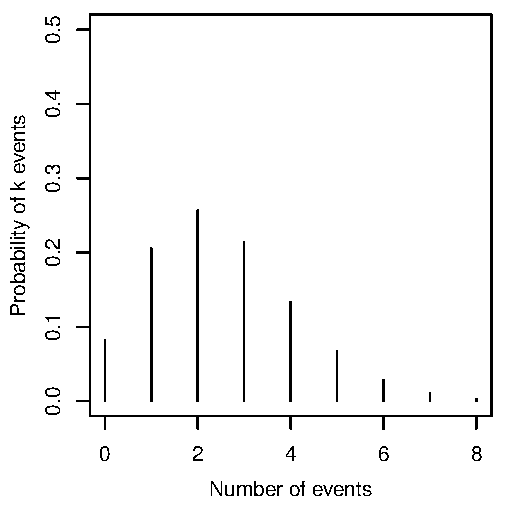
\includegraphics[scale=.7]{../figures/pois_dist}
  \end{center}
\end{column}
\begin{column}{.5\textwidth}
  \begin{lstlisting}
x <- 0:8
px <- dpois(x, lambda = 2.5)
plot(px ~ x, type = "h")
\end{lstlisting}
\end{column}
\end{columns}
\end{frame}

\begin{frame}{Poisson regression}

Poisson regression is used to model count variables\footnote{Simulated dataset from
  \url{https://stats.idre.ucla.edu/stat/data/poisson_sim.csv} \citep{UCLAstats}}\\[2ex]
\begin{columns}[c]
\begin{column}{.5\textwidth}
  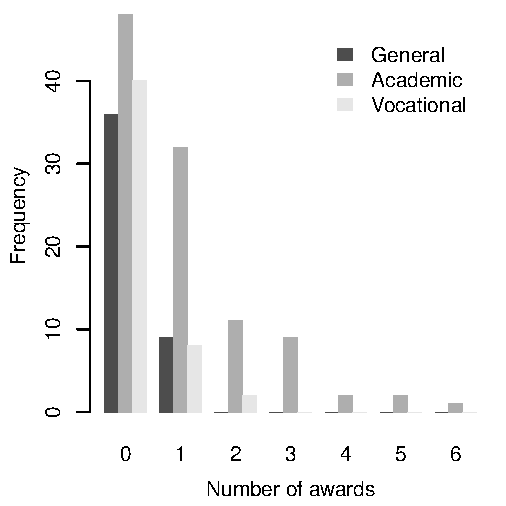
\includegraphics[scale = .65]{../figures/pois_example}
\end{column}
\begin{column}{.5\textwidth}
  Variables
  \begin{itemize}
    \item Number of awards earned by students at one high school
    \item Type of program in which student was enrolled (vocational,
    general, or academic)
    \item Score on students' final exam in math
  \end{itemize}
\end{column}
\end{columns}
\end{frame}

\begin{frame}{Poisson regression}
  \begin{itemize}
    \item We estimate a poisson regression using a generalized linear model
      with \texttt{family = poisson} and link function \texttt{log}
  \begin{align*}
    g(E(y)) & = \beta_0 + \beta_1 x_1 + \beta_2 x_2\\
    \log(\mu) & = \beta_0 + \beta_1 prog + \beta_2 math
  \end{align*}
  with $y_i \sim \text{Poisson}(\lambda)$
  \end{itemize}
\end{frame}

\begin{frame}[fragile]{Poisson regression}
  \begin{lstlisting}
# Read data
dat <- read.csv("poisson_sim.csv")

# Define factors
dat$prog <- factor(dat$prog, levels = 1:3,
                   labels = c("General", "Academic", "Vocational"))
dat$id <- factor(dat$id)

# Fit poisson regression
m1 <- glm(num_awards ~ prog + math, family = poisson, data = dat)
summary(m1)

# Evaluate goodness-of-fit
1 - pchisq(m1$deviance, df = m1$df.residual)
\end{lstlisting}
\end{frame}

\begin{frame}{Poisson regression}
\begin{itemize}
  \item The results show that the model fits the data with $G^2(196) =
    189.45,~p=0.6182$
  \item The expected number of awards when in the academic program is
    $\exp(1.0839) = 2.96$ times the expected number for the general program
    when math grade is held constant
  \item The expected number of awards increases by a factor of
    $\exp(0.0702) = 1.07$ when math grade increases by one unit (and
    program is held constant)
\end{itemize}
\end{frame}

\begin{frame}{Predictions of the poisson regression}
\begin{columns}[c]
\begin{column}{.5\textwidth}
  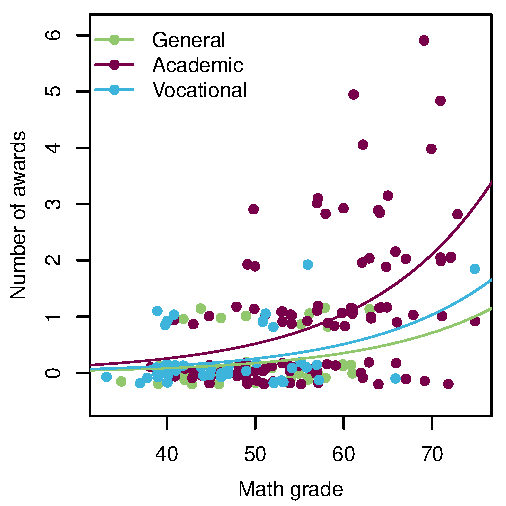
\includegraphics[scale=.7]{../figures/pois_pre}
\end{column}
\begin{column}{.5\textwidth}
  Variables
  \begin{itemize}
    \item Number of awards earned by students at one high school
    \item Type of program in which student was enrolled (vocational,
    general, or academic)
    \item Score on students' final exam in math
  \end{itemize}
\end{column}
\end{columns}
\end{frame}

\section{Overdispersion}

\begin{frame}{Overdispersion}
  \begin{itemize}
    \item Overdispersion is the presence of greater variability in a data
      set than would be expected based on a given statistical model
    \item It means that the underlying distributional assumptions might be
      violated
    \item The binomial and the poisson distribution are both less flexible
      than, e.\,g., the normal distribution, since they only have one free
      parameter and, therefore, the variance cannot be adjusted
      independently of the mean
    \item We can include a so-called overdispersion parameter $\varphi$
      into both models
    \item For the poisson regression, instead of assuming $E(y) = Var(y) =
      \mu$, we model $Var(y) = \varphi\mu$
  \end{itemize}
\end{frame}

\begin{frame}[fragile]{Overdispersion}
  \begin{itemize}
    \item In R this is done by changing the \texttt{family} argument to
      \texttt{quasibinomial} or \texttt{quasipoisson}.
  \end{itemize}

%small change

  \vfill
\begin{lstlisting}
# Fit poisson regression
m2 <- glm(num_awards ~ prog + math, family = quasipoisson, data = dat)
summary(m2)

# --> Results show that estimated parameters are still the same,
# but standard errors are slightly higher
\end{lstlisting}
\end{frame}

\begin{frame}{Some things to consider}
  \begin{itemize}
    \item When using \texttt{family = "quasipoisson"} or \texttt{family =
      "quasibinomial"}, likelihood-ratio tests are not meaningful anymore
      (even though R will let you do them)
    \item Goodness-of-fit tests are not necessarily meaningful for
      \emph{continuous} predictors for poisson and binomial regression, so
      use with caution
      (see, e.\,g.,
      \url{http://thestatsgeek.com/2014/04/26/deviance-goodness-of-fit-test-for-poisson-regression/})
  \end{itemize}
\end{frame}


\begin{frame}[fragile]{}
  \begin{block}{Exercise\footnote{Inspired by \url{https://rstudio-pubs-static.s3.amazonaws.com/1047952_9306ae04c1de4543812af559d777dd72.html}}}
    \begin{itemize}
      \item Fit a regression model to the \texttt{Affairs} data set from the
        \texttt{AER} package in R
      \item The variable \texttt{affairs} is the number of extramarital affairs
        in the past year and is our response variable
      \item Include the variables \texttt{gender}, \texttt{age},
        \texttt{yearsmarried}, \texttt{children}, \texttt{religiousness},
        \texttt{education} and \texttt{rating} as predictors
      \item \texttt{religiousness} ranges from 1 (anti) to 5 (very) and
        \texttt{rating} is a self rating of the marriage, ranging from 1 (very
        unhappy) to 5 (very happy)
      \item Assess the Goodness-of-fit using the deviance
      \item Assess overdispersion and decide if a model with an extra dispersion
        parameter might be indicated
      \item Compare the confidence intervals for the estimated parameters for
    both models \end{itemize}
  \end{block}
\end{frame}

\appendix

%\begin{frame}[allowframebreaks]{References}
\begin{frame}{References}
  \printbibliography
  \vfill
\end{frame}

\end{document}

